% The main file for my thesis
% each \textbf{chapter} is included from this main file
\documentclass[11pt,a4paper]{uolthesis}
%\documentclass[11pt,a4paper]{article}
%\usepackage{alltt,float}
%\usepackage{lgrind}
\usepackage{url}                    % for better handling of URL
\usepackage{lscape}                 % allow to use \begin{landscape}, which makes a page in landscape.
%\usepackage{subfigure}
\usepackage{mathrsfs}
\usepackage{graphicx}
%\usepackage{caption2}
\usepackage{epstopdf}
\usepackage{apacite}
\usepackage{natbib}
\usepackage{amsmath}
\usepackage{tikz}
\usepackage{pgfplots}
\usepackage{caption}
\usepackage{subcaption}
\usepackage{pgfgantt}
\usepackage{multirow}

\usetikzlibrary{shapes.arrows}

\newcommand{\citepos}[1]{\citeauthor{#1}'s \citeyearpar{#1}}
\newcommand{\citeposs}[1]{\citeauthor{#1}' \citeyearpar{#1}}

%Modify the Figure Captionequ1-1:shannon
%\renewcommand{\figurename}{Fig.}
%set the figures captions
%\captionstyle{hang} \setcaptionwidth{13cm}
%**********************************************

% correct bad hyphenation here
\hyphenation{op-tical}
% use less hyphenation
\lesshyphenation
% or totally stop it
%\nohyphenation

% include them only, as I am currently working on them
%\includeonly{ch1/ch1}

% begin the main document
\begin{document}

% include the title pages, acknowledgements, and author's publications

\title{A Geometric Method for Context Sensitive Distributional Semantics}

\author{Stephen McGregor}
\department{School of Electronic Engineering and Computer Science} \college{Queen Mary, University of London}
\degree{Doctor of Philosophy} \degreemonth{September} \degreeyear{2017}

%% By default, the thesis will be copyrighted to MIT.  If you need to
%% copyright the thesis to yourself, just specify the `vi' documentstyle
%% option.  If for some reason you want to exactly specify the copyright
%% notice text, you can use the \copyrightnoticetext command.
%\copyrightnoticetext{\copyright ~University of London, 2006}

% The dedication info.
%\dedication{TO MY FAMILY}

% Make the titlepage based on the above information.  If you need something
% special and can't use the standard form, you can specify the exact text of
% the titlepage yourself.  Put it in a titlepage environment and leave blank
% lines where you want vertical space. The spaces will be adjusted to fill
% the entire page. The dotted lines for the signatures are made with the
% \signature command.

% Make the first title page
\maketitle

% make the dedication page
%\makededication

\makedeclaration

% Start to count page number from abstract page
\pagestyle{plain}%
\setcounter{page}{1}
\pagenumbering{roman} %

% The abstractpage environment sets up everything on the page except the
% text itself.
%
% You can either \input (*not* \include) your abstract file, or you can put
% the text of the abstract directly between the \begin{abstract} and
% \end{abstract} commands.
\begin{abstract}
%\input{abstract}
% abstract goes here
This thesis describes a novel methodology, grounded in the distributional semantic paradigm, for building context sensitive models of word meaning, affording an empirical exploration of the relationship between words and concepts. Anchored in theoretical linguistic insight regarding the contextually specified nature of lexical semantics, the work presented here explores a range of techniques for the selection of subspaces of word co-occurrence dimensions based on a statistical analysis of input terms as observed within large-scale textual corpora. The relationships between word-vectors that emerge in the projected subspaces can be analysed in terms of a mapping between their geometric features and their semantic properties. The power of this modelling technique is its ability to generate ad hoc semantic relationships in response to an extemporaneous linguistic or conceptual situation. 

The product of this approach is a generalisable computational linguistic methodology, capable of taking input in various forms, including word groupings and sentential context, and dynamically generating output from a broad base model of word co-occurrence data.  To demonstrate the versatility of the method, this thesis will present competitive empirical results on a range of established natural language tasks including word similarity and relatedness, metaphor and metonymy detection, and analogy completion. A range of techniques will be applied in order to explore the ways in which different aspects of projected geometries can be mapped to different semantic relationships, allowing for the discovery of a range of lexical and conceptual properties for any given input and providing a basis for an empirical exploration of distinctions between the semantic phenomena under analysis. The case made here is that the flexibility of these models and their ability to extend output to evaluations of unattested linguistic relationships constitutes the groundwork for a method for the extrapolation of dynamic conceptual relationships from large-scale textual corpora. 

This method is presented as a complement and a counterpoint to established distributional methods for generating lexically productive word-vectors. Where contemporary vector space models of distributional semantics have almost universally involved either the factorisation of co-occurrence matrices or the incremental learning of abstract representations using neural networks, the approach described in this thesis preserves the connection between the individual dimensions of word-vectors and statistics pertaining to observations in a textual corpus. The hypothesis tested here is that the maintenance of actual, interpretable information about underlying linguistic data allows for the contextual selection of non-normalised subspaces with more nuanced geometric features. In addition to presenting competitive results for various computational linguistic targets, the thesis will suggest that the transparency of its representations indicates scope for the application of this model to various real-world problems where an interpretable relationship betweendata and output is highly desirable. This, finally, demonstrates a way towards the productive application of the theory and philosophy of language to computational linguistic practice.

\end{abstract}

% Acknowledgments
%
% You can either \input (*not* \include) your acknowledgments file, or you can put
% the text of the acknowledgments directly between the \begin{acknowledgments} and
% \end{acknowledgments} commands.
%\begin{acknowledgments}
%\input{acknowledgments}
%Acknowledgment goes here...

%\end{acknowledgments}

%\begin{context}
%The term \emph{context} has been used widely and variously by authors in both theoretical and computational linguistics, and with good reason, as various sense of the concept of context are clearly at play in any serious discussion of the interplay between language and cognition.  Statistically minded computational linguists in particular, of whom I would like to count myself as one, have often used \emph{context} to refer to the window of co-occurrence in which a word token is observed within a sample of text.  In his description of a co-occurrence statistic for measuring semantic similarity, \cite{Salton1992b} introduced the term \emph{context space} to refer to a space of co-occurrence dimensions, a terminology subsequently adopted by \cite{BurgessEA1997} in relation to their HAL system.  This notion of proximity within a text as context has persevered in the natural language processing literature.

%Theoretical linguists and cognitive scientists, on the other hand, have tended to treat \emph{context} as a thing 

%So 

%and this nomenclature has been carried on by subsequent researchers interested in the idea that cognition, conceptualisation, and, correspondingly, language are always in some way specified by a situation in the world.

%In this thesis, I will endeavour to use the term \emph{context} strictly in reference to the latter notion of 

%\end{context}

\begin{glossary}
\begin{description}
\item[base space] A high dimensional, sparse vector space of word-vectors, delineated in terms of dimensions of co-occurrence statistics.
\item[context] The situation -- environmental, cognitive, perceptual, linguistic, and otherwise -- in which an agent finds itself and applies language to meaning.
\item[contextual input] A set of words characteristic of a conceptual category or semantic relationship used to generate a subspace for the modelling of semantic phenomena.
\item[dimension selection] The process of contextually choosing a subset of dimensions in order to project a subspace from a base space.
\item[co-occurrence] The observation of one word in proximity to another in a corpus.
\item[co-occurrence statistic] A measure of the tendency for one word to be observed in proximity to another across a corpus.
\item[co-occurrence window] The boundary defining the proximity within which two words are considered to be co-occurring, typically a distance in terms of words within a sentence.
\item[methodology] The process of building base spaces from observations of co-occurrences within a corpus and contextually projecting subspaces through dimension selection.
\item[model] An application of methodology to a particular linguistic task or experiment, sometimes including task specific statistical analysis techniques.
\item [subspace] A context specific lower-dimensional projection from a base space, effectively mapping semantic relationships to a context by way of the geometric relationships between word-vectors.
\item[word-vector] A high-dimensional geometrically situated semantic representation of a word, constructed as an array of co-occurrence statistics.
\end{description}
\end{glossary}


%\include{format}
% Generate table of contents and the list of figures, tables and abbreviations
\tableofcontents
%% create the toc, lof, and lot, they are added into toc by tocbibind package
\tableofcontents   % Create Table of Contents
\listoffigures     % Create List of Figures%
\listoftables      % Create List of Tables%

\iffalse
List of Abbreviations
\chapter*{List of Abbreviations}
  \addcontentsline{toc}{chapter}{List of Abbreviations}
\begin{tabular}{ll}
\\
3D & Three-Dimensional\\

3G & Third Generation\\

3GPP & Third Generation Partnership Project\\

4G & Fourth-Generation\\

A-GPS & Assisted-GPS\\

AOA & Angle of Arrival\\

AWGN & Additive White Gaussian Noise\\

BLAST & Bell Labs Layered Space Time\\

BT & Base Station\\

CA & Circular Array\\

CDF & Cumulative Distribution Function\\

DECT  &  Digital Enhanced Cordless Telecommunications\\

DF & Degradation Factor\\

DLR & German Aerospace Centre\\


DR & Dielectric Resonator\\

EU  & European Commission \\


EVD & Eigen Value Decomposition \\

GAC & Galileo Advanced Concept\\



\\
\end{tabular}


\begin{tabular}{ll}
\\

GJU & Galileo Joint Undertaking\\

GO & Geometrical Optics\\

GPS & Global Positioning System \\

GSM & Global System for Mobile Communications\\

GTD & Geometrical Theory of Diffraction\\

IEEE & Institute of Electrical and Electronics Engineers\\

IFA & Inverted-F Antenna\\

iid & independent and identically distributed\\

ILA & Inverted-L Antenna\\

IP & Internet Protocol\\

IST & Information Society Technologies\\

LTE & Long Term Evolution\\

MIMO & Multiple Input Multiple Output\\

MT & Mobile Terminal\\

NLOS & Non-line-of-sight\\

NMHA & Normal Mode Helix Antenna\\

OFDM & Orthogonal Frequency Division Multiplexing\\

PCS  & Personal Communication Services\\

PDA & Personal Digital Assistant\\

PDC & Personal Digital Communications\\

PIFA & Planar Inverted-F Antenna\\

QMUL & Queen Mary, University of London\\

RF & Radio Frequency\\

RHCP & Right Hand Circular Polarisation\\

RT & Ray Tracing\\

Rx & Receiver \\






\\
\end{tabular}

\begin{tabular}{ll}
\\

SBR & Shooting and Bouncing Ray\\

SC & Selection Combiner\\

SIMO & Single Input Multiple Output\\

SISO & Single Input Single Output\\

SNR & Signal-to-noise ratio\\

SVD & Singular Value Decomposition\\

Tx & Transmitter\\

ULA & Uniform Linear Array \\


UTD & Uniform Theory of Diffraction\\


UTD & Uniform Theory of Diffraction\\

WiMAX & Worldwide Interoperability for Microwave Access\\

WLAN & Wireless Local Area Network\\

WP & Work Package\\

XPR & Cross-polar ratio\\



\\
\end{tabular}
\fi

\newpage

% begin of main text
\setcounter{page}{1} %
\pagenumbering{arabic}
% enable the headers
\pagestyle{fancy}


%\setcounter{chapter}{-1}
%\setcounter{page}{1}
%\pagenumbering{arabic}

% Start the main context
%\setcounter{page}{1}
\pagenumbering{arabic}

\chapter{Preamble: Stage 2 Report}
This document presents the state of my PhD research as I enter the third year of my studies at Queen Mary.  My research project will be introduced properly in Chapter 1.  This preliminary chapter serves simply to introduce this document, which I hope will serve as the kernel of a full dissertation.  The following sections will lay out the work accomplished to date, both in terms of publications and experiments, and will also project the work that lies ahead over the next 18 months.  The rest of this document will hopefully serve as a template for the final presentation of my PhD, both as an outline and as a guide for the work the remains to be done.  No section is even close to complete, and some, particularly later in the document, are essentially empty, as the bulk of evaluative work on this project is pending.

\section{Completed, Ongoing, and Future Publications}
I've published five conference papers to date, with a potential forthcoming journal publication currently undergoing a first round of revision.  \cite{McGregor2014} explores the relationship between computational creativity and intellectual property law, and, in so doing, drew out some of the inherent difficulties in evaluating the output of a symbol manipulating system in terms creativity.  Related theoretical work was presented in \cite{McGregorEA2014}, where we address the philosophically problematic relationship between cognition and mental representation from the perspective of the analysis of creativity.  An idea central to my PhD work emerges from these two early papers: in order for the behaviour of an agent to be perceived as creative, the agent must offer an observer at least the facsimile of some sort of system of internal representations that dynamically interact with each other and with the environment to produce artefacts.

\cite{McGregorEA2015} continues in a philosophical vein, raising questions about the emergence of the type of goal-directed behaviour that is often taken to be implicit in acts of creation.  Again with a thoroughly theoretical grounding, \cite{McGregorEA2015b} introduces an overview of some of the computational approaches that will be used to map between geometric representations of conceptual spaces by way of generating interesting new metaphors.  The idea of using the geometric properties of distributional semantic models to perform metaphoric mappings was also presented by me at a talk at ICLC this past summer, though the talk was accompanied by an abstract rather than a full paper, as seems to be the norm with theoretical linguistic conferences.  In a much more empirically oriented paper, \cite{AgresEA2015} outlines for the first time the methodology for building a high-dimensional statistical language model which can be used to project conceptual subspaces in a momentary, contextually informed way.  This practical work is pushed further in \cite{McGregorEA2015c}, with an in-depth description of the model and further experiments designed to reveal its ability to map from language to contextually nuanced conceptual spaces.

My plan for the months ahead, in terms of research and corresponding publication, is to expand the headway made in the work published thus far towards the completion of two general tasks with a well established history in the computational linguistic literature: taxonomy recapitulation and analogy completion.  The general approach to analogy completion has already been outlined in \cite{McGregorEA2015b}, and I think we're getting close to the point where the model will be ready to handle some of the existing test sets for this type of task.  In terms of the construction of lexical ontologies, this kind of process is even more immediately inherent in the work already presented in \cite{AgresEA2015,McGregorEA2015c}.  With regard to these two anticipated results, I envision targeting some of the major summertime computational linguistic conferences such as ACL and EMNLP with highly empirical articles, and imagine there would also be ample material for one or two subsequent journal articles pending strong results.

\section{Schedule for the Next 18 Months}
What has been accomplished so far is the design and implementation of a contextually sensitive distributional semantic language model.  Ongoing experiments are confirming the hypothesis that this model is good at returning clusters of words which can be mapped as conceptual constituents.  The way forward for using this model for constructing lexical ontologies (ie, taxonomies) seems fairly clear.  Early experiments comparing the geometries of word clusterings within different spaces suggests that the intuition that congruence should provide a mechanism for analogy completion have also returned fairly positive results.

Following on this continued investigation, I plan on spending some time considering ways in which the dimensional reduction process might be described in a more mathematically rigorous way---my hunch at the moment is that there might be a way to consider this aspect of the model's operation in terms of a Laplacian matrix or perhaps a Riemannian manifold, but I need to do considerably more research in this direction.  It would be nice to have a more mathematically rigorous way of describing the model.  For the time being this notion remains speculative, so I will not include it in the thesis outline that follows, but it would be a nice way of objectifying some of the work that's already been done and so in my opinion deserves further consideration.

The two well-defined targets for the months ahead, taxonomy recapitulation and analogy completion, each culminate in a conference paper deadline.  Some conceptual work remains to be done: the way that the model speculates about seed clusters for different sense of a hypernymic term is under development, and the mechanism for exploring the geometry of clusters within subspaces likewise requires further investigation.  These experimental exercises will lead on to the development of the model's metaphor generating facilities, which will serve as the basis for the ultimate demonstration of the strength of this project as a practical exposition of a theoretical stance on the nature of language.

\begin{figure}[t]
	\caption{Scheduling for the Final 18 Months}
	\scriptsize
	\begin{center}
		\begin{ganttchart}[vgrid={*{30}{white},*{1}{black,dotted},*{29}{white},*{1}{black,dotted},*{30}{white},*{1}{black,dotted},*{30}{white},*{1}{black,dotted},*{28}{white},*{1}{black,dotted},*{30}{white},*{1}{black,dotted},*{29}{white},*{1}{black,dotted},*{30}{white},*{1}{black,dotted},*{29}{white},*{1}{black,dotted},*{30}{white},*{1}{black,dotted},*{30}{white},*{1}{black,dotted},*{29}{white},*{1}{black,dotted}},hgrid,x unit=0.2mm,y unit chart=5mm,time slot format=isodate,link bulge=10,link tolerance=300,group peaks width=10,group peaks tip position=0,bar/.append style={fill=gray},bar label font=\scriptsize]{2015-10-01}{2017-03-30}
			\gantttitlecalendar{year,month} \\
			\ganttgroup{Parameters}{2015-10-01}{2016-01-01} \\
			\ganttbar[name=Jagi]{JAGI}{2015-10-01}{2015-10-19} \\
			\ganttbar[name=ParT]{Tweeking}{2015-10-01}{2015-12-01} \\
			\ganttbar[name=ParF]{Formalising}{2015-11-01}{2016-01-01} \\

			\ganttgroup{Taxonomy}{2015-10-01}{2016-03-01} \\
			\ganttbar[name=TaxT]{Testing}{2015-10-01}{2016-02-15} \\
			\ganttbar[name=TaxW]{Writing}{2016-02-01}{2016-03-01} \\

			\ganttgroup{Analogy}{2015-10-19}{2016-06-01} \\
			\ganttbar[name=AnaF]{Festival}{2015-10-19}{2015-11-14} \\
			\ganttbar[name=AnaT]{Testing}{2016-02-01}{2016-05-15} \\
			\ganttbar[name=AnaW]{Writing}{2016-05-01}{2016-06-01} \\

			\ganttgroup{Metaphor}{2016-02-01}{2016-08-01} \\
			\ganttbar[name=Deve]{Development}{2016-02-01}{2016-08-01} \\

			\ganttgroup{Evaluation}{2016-04-01}{2016-11-01} \\
			\ganttbar[name=EvaS]{Social Media}{2016-04-01}{2016-11-01} \\
			\ganttbar[name=EvaH]{Subjects}{2016-06-01}{2016-10-01} \\

			\ganttgroup{Writing}{2016-07-01}{2017-01-01} \\
			\ganttbar[name=WriL]{Theory}{2016-07-01}{2016-10-01} \\
			\ganttbar[name=WriI]{Meth \& Imp}{2016-09-01}{2016-11-01} \\
			\ganttbar[name=WriR]{Results}{2016-10-01}{2016-12-01} \\
			\ganttbar[name=WriE]{Eval \& Conc}{2016-11-01}{2017-01-01} \\
			
%			\ganttlink{ParT}{ParF}
%			\ganttlink[link bulge=270,link mid=0.35]{ParF}{WriI}
%			\ganttlink{TaxT}{TaxW}
%			\ganttlink[link bulge=200,link mid=0.55]{TaxT}{WriR}
%			\ganttlink{AnaT}{AnaW}
%			\ganttlink[link bulge=30]{AnaT}{Deve}
%			\ganttlink[link bulge=200,link mid=0.55]{AnaT}{WriR}
%			\ganttlink[link bulge=105]{Deve}{EvaS}
%			\ganttlink[link bulge=105]{Deve}{EvaH}
%			\ganttlink{Deve}{WriI}
%			\ganttlink[link bulge=135]{EvaS}{WriE}
%			\ganttlink{EvaH}{WriE}
		\end{ganttchart}	
	\end{center}
\end{figure}

\chapter{Introduction}
In Italo \citepos{Calvino1983} whimsical novel of ideas \emph{Mr. Palomar}, the titular character reflects upon the mating rituals of turtles.  Encased as they are in an unfeeling shell, with only a filament of sensing flesh with which to prod the world, Palomar concludes that for turtles sensuality must take on an almost entirely cerebral aspect: ``The poverty of their sensorial stimuli perhaps drives them to a concentrated, intense mental life, leads them to a crystalline inner awareness,'' (p. 18).

The chelonian condition imagined by Palomar is, at least in a certain metaphoric respect, the endemic situation of a statistical language model.  The environment of such a model is at best a sparse simulacrum of existence, a trickle of information that is only about anything in a sense completely external to the model itself.  If language is characterised by an aboutness that anchors itself in acts, intentions, and experiences in the world, then the blind traversal of corpora severs the semantic anchor lines and allows a model to curl into itself.  The residue of this process, an accumulation of symbols trailed by kite tails of numbers, can really only be directly interpreted as an echo of language, revealing tendencies but demanding clever interpretive reconstruction in order to be of any practical use.

This thesis sets out to explore the question of if and how a statistical language model can be involved in the generation of new meaning.  That such models can at least be interpreted in a way that compellingly exposes semantic and syntactic relationships has been demonstrated, and the trend in ongoing work in this area is to continue to develop mechanisms for recapitulating datasets while allowing the features of the models themselves to drift further away from semantic transparency.  The positive outcome is a battery of computationally tractable and sometimes mathematically elaborate mechanisms for processing natural language, some of which appear to have real practical applications in tasks such as information retrieval and machine translation.  There is a risk, however, of a proliferation of models that are very good at solving bespoke micro-problems but reveal very little about the nature of language.

One of the objectives of this work, then, is to explore the relationship between the abstract geometry of relatively high-dimensional language models and the concrete geometry of the world that language must be about.  \cite{Kant} places the geometric representation of the world at the foundation of mental existence, classing it in terms of fundamental \emph{intuitions} rather than supervenient \emph{concepts}.  Already a parallel between language and conceptualisation is emerging here: concepts are about space, and also somehow composed of space, in the way that words are the world and also in the world.

When words become points, the language itself, consisting of those words and the relationships between them, becomes a spatial entity, but in an abstract space where there is not even a nominal distinction between space and information.  It is no longer a space in the essential sense of Kant, but rather a generative space, a space that is somehow an index to that other space which is co-extensive with reality.  In this kind of space, it is the space itself that does the work: it is the space that comes to characterise the features of each point, and, when points interact, they interact by virtue of nothing other than their positions.  When a statistical language model is interpreted, it is therefore the internal space of the web of relationships working as a dynamic system unto itself that are being explored.

This thesis seeks to ground these philosophical arguments in computational experimentation.  The methodology described and pursued in the following pages finds its motivation in theoretical considerations of language and cognition, but its techniques are rooted in the contemporary approach to statistical language modelling.  The unique contribution of the model that will be described here, though, is to offer a robust mechanism for the prolific contextualisation of the lexical information inherent in the network of statistics that delineate its spatial aspect.  In this regard, what is being modelled is the relationship between language and concepts as they come about in the world, in the unfolding, ready-to-hand, non-sentential character of cognition.

With that said, no strong claim will be made here about having resolved the hard questions surrounding the mind.  There is no suggestion that the model described in this thesis is somehow simulating cognition; indeed, the mechanism of a computational model such as this, substantiated by nothing more than the drizzle of data that penetrates its shell, is specifically different than the way a cognitive agent evolves into a situation of deep, tight, multifarious entanglement with the world.  Furthermore, it is essential not simply to dismiss the challenges that face any attempt at a philosophically robust description of cognition.  Indeed, these philosophical problems will become a guiding light for this work, with the hope that a good model that is honest about the level of abstraction at which it is applicable may reveal some interesting aspect of the elaborate whole.

The strong claim which will be made is that the model described here can participate autonomously in the discovery of new and useful meaning, and it is in this regard that this work finds its roots in the multifaceted field of computational creativity.  When \cite{Wittgenstein} states that ``only the act of meaning can anticipate reality'' (p. 76), he suggests that beyond a mere syntactic encoding of events in the world, language is tied up in a process of connecting mental existence to being in the world.  Creativity, construed as meaning making, is taken as a broad target for a project that attempts to model the semantics inherent in the relationship between words and concepts.  The work presented here does not aspire to the kind of phenomenological richness that is at the heart of Wittgenstein's later philosophy, but it has been designed to generate informational structures that might be interpreted as models of internal representations with the interactional dynamics necessary for generating significant new meaning.

So, while there may be a popular perception that figurative language is in some regard more creative than plainly propositional language, the choice of metaphor as a target is actually motivated by the way in which figurative language exposes the functionality of words.  In the course of constructing a metaphor, a linguistic agent is seeing meaning as an affordance for some communicative action: just as a shoe might become a hammer, or a chair a weapon, the concept of a butcher comes to stand in for a certain type of surgeon in a certain context.  It is this opportunism inherent in language which the project presented here will attempt to model.

\section{A Hypothesis}
The premise of this this thesis is that conceptualisation can be modelled in geometric terms, not least because concepts are about a reality that is essentially geometric.  Furthermore, the relationship between concepts and language is to be discovered in the way that language is in the world: language is about the world, but it is also made of the world, and the relationship between the two is as determinate as it is irretrievable.  When language comes about as an affordance of communication, it is a physical opportunity for expressive action that is being directly perceived as an aspect of an environment, as a way to use and change that environment.  The situation of language is inextricably spatial and functional, and so the language itself can only really properly be modelled as something that is dynamic and geometric.

Following on this, the hypothesis offered here is that figurative language can be modelled in terms of the geometrical properties of a statistical language model.  In particular, this paper predicts that a dynamically generative distributional semantic model, equipped with a facility for projecting contextually informed subspaces from a base lexical space, will remit clusterings of word-vectors that can be interpreted as geometric representations of conceptualisations, and the work to be described in the following chapters is predicated upon this prediction.  A significant consequence of the geometric modelling of concepts is that the geometric properties of these conceptually charged word spaces will allow for the isomorphic mapping between conceptual representations as a methodology for modelling the generation of figurative language based on contextually specific information.

By way of testing this hypothesis, a statistical language model will be developed and subjected to a set of experiments.  In particular, the model will be tested in terms of established approaches to the recapitulation and extension of lexical ontologies and to the completion of analogies.  Furthermore, in an effort to test the pragmatic efficacy of the model, metaphoric output will be measured in a study involving human subjects and also, through a social media application of a metaphor generating bot, submitted to the tumult of public discourse.  The purpose of this final measure is to test the pragmatic applicability of the model's output in a real communicative situation.  It is by virtue of this last point in particular that this remains fundamentally a thesis about computational creativity, in that the trafficking of statements produced by an on-line application will be taken as affirmation that the behaviour of a system associated with the model has been interpreted as essentially creative in its generation of new, useful language.

\section{Contributions to the Field}
The concrete manifestation of the work described here is a system for generating conceptual metaphors: given linguistic input describing a basic situation in the world, for instance, ``that surgeon is sloppy'', the system will return a figuratively loaded description such as ``that surgeon is a butcher''.  The mechanism involved in discovering such new relationships between conceptual entities employs dynamically interactive representations, in that the mathematical, geometric nature of the model's word-labelled representations provides a platform for intermeshings which might lead to the emergence of representations that are dynamic on a conceptual level.  As such, from the perspective of computational creativity, there is a case to be made that something like internal representations of conceptual schemes are being modelled, and it will be argued here that this model can be considered in terms of the autonomous generation of novel, compelling linguistic artefacts through a process that can be deemed creative.

A similarly concrete but broader contribution of this work is the presentation of a new language model, specifically engineered to handle the nuance of conceptualisation that the pragmatics of natural language capture so well.  More than just another new model for performing a range of NLP type tasks, the goal here is to provide an endorsement for a particular type of model, namely, one that maintains features that are, in a statistical sense, interpretable as actual informational observations.  As \cite{White2009} has put it, ``we need some sort of cognitive grasp'' (p. 99) on the way in which statistical techniques tease a semantic model out of large scale corpora.  The work presented here is designed as a transparent implementation of a theory about the contextualisation involved in mapping from words to concepts, and so the expectation is that this might at least indicate a methodological stance for achieving this cognitive desideratum.

Finally, on a more abstract level, this work is offered as an indication of one way in which computers might be used to empirically demonstrate the efficacy of philosophical arguments.  In particular, the model presented here takes a theory about the nature of language and the contextual way in which language becomes deeply entangled with conceptualisation, and it applies this theory to an exercise in the design and testing of a model.  One of the broad aspirations of this dissertation is to hint at a way in which future work in both computer science and philosophy can seek a harmonious balance between theory and practice.  This is offered as something of an antidote to the fraught relationship between the philosophy of mind and the application of computer modelling, which has been persistently hampered by very reasonable objections to the erroneous claim that minds and computers are somehow just like each other.  The counterargument offered here is that minds and computers are fundamentally different, but there is still much to be gained in terms of both insight and application from using computers to model some of the things -- language, conceptualisation, creativity -- that are clearly native to the mind.  The key here is to keep in mind certain truths about the physical and, on the other hand, observer dependent nature of computing, and not to lose sight of the level of abstraction at which computational models can be understood.

\section{Structure of The Dissertation}
In addition to this introductory chapter, this thesis contains six more chapters.  The second chapter will present a review of relevant literature, both in terms of historical theoretical material and contemporary empirical work in the several fields related to this project.  This literature review will be followed by an exposition of the theoretical foundation of the project itself, describing the conceptual basis for the experimental work that will subsequently be described.

The fourth chapter will lay out the methodological approach to the construction of a generative language model, as well as the equations describing the mechanism for using this base model to project contextually informed subspaces.  It will also describe techniques for taxonomy recapitulation and the discovery of conceptual metaphors by way of mapping between word clusters discovered in the base model's projections.  The fifth chapter will describe the implementation of the language model, including its application to tasks involving completion of established test sets and recapitulation of widely used lexical ontologies.  Results of these experiments will also be presented in this chapter.

The sixth chapter will discuss the experimental results presented in the previous chapter from an analytical perspective.  Additionally, this chapter will present two further mechanisms for evaluating the model's metaphor generating capabilities in particular, in terms of a study involving human subjects and a pragmatically geared application of social media.  The seventh and final chapter will provide a holistic diagnosis of the project, returning in particular to the philosophical ambitions of this work and also considering potential future applications of the model.

\chapter{Background}
The ambitious scope of this project requires a thorough grounding in the literature from a range of disciplines.  The risk in such an inclusive undertaking is that there are many opportunities for going astray.  The reward, a piece of empirical work that exemplifies the possibility of using computers to do theoretically significant research, seems to justify the risk, but only if the final product is well placed in the context of existing work in the area.  The following chapter will delineate the territory that this thesis seeks to explore, by way of a survey of the considerable canon of theoretical work relating to the problems of minds, concepts, and language as well as the increasingly substantial body of practical work on computational linguistics and its application to the modelling of creative language generation.

\section{Computers and Creativity}
At its heart, this is a project about the potential for symbol manipulating machines to model creativity, and in particular the creative use of language.  Computational Creativity is a field that, as \cite{Wiggins2006b} puts it, uses ``computational means and methods'' to study ``behaviour exhibited by natural and artificial systems, which would be deemed creative if exhibited by humans,'' (p. 210).  At stake here is the problem of what creativity actually is, and, as \cite{Colton} have said, the concept of creativity must be \emph{essentially contested}.  Nonetheless, a basic position will be taken here that at the root of creativity is, in the spirit of \cite{Wittgenstein1953}, an act of meaning-making, by which a new way of conceptually representing something in the world comes about.

The prevalent take on computational creativity has focused on an AI approach involving the traversal of state spaces for potential creative artefacts, a methodology with deep roots in \cite{Boden1990}.  Philosophical problems with this essentially symbolic mode of generation have been illustrated by \cite{McGregorEA2014}, though: the dependency on preconditioned representations remits little in the way of actual creative behaviour on the part of the symbol manipulating agent.  Here the hard question of evaluation comes up, and the evaluative challenges peculiar to computational creativity have been addressed by \cite{Ritchie2007}, \cite{ColtonEA2012B}, and \cite{Jordanous2012}, to name a few.  At the core of this project is the proposal that, for an agent to be perceived as genuinely and autonomously instigating meaning-making, there has to be at least a nominal notion of the trafficking of dynamic, interactive representations within the agent's cognitive framework.  It is here that computational creativity will serve as a compass to keep this project on course: by returning to the question of whether the model outlined here can be described as an agent that is behaving creatively, the pragmatic issue of the role of contextualisation in the actual use of language will stay central to the thesis.

In addition to a general survey of the field, this project's particular commitment to conceptualisation and metaphor invites a survey of the appreciable work done in the computational production of metaphor and analogy.  With roots in the conceptual blending theory of \cite{Turner}, this area has been explored more recently by the likes of \cite{VealeEA2007} and \cite{O'Donoghue}.  Additional attention is due to work in poetry generation coming from \cite{Gervas}, \cite{Toivonen}, \cite{Rashel}, \cite{Cardosa}, and others.

\section{Minds and Spaces}
\cite{Davidson} cautions against considering language as an ``organising system'' (p. 11) for conceptual schemes.  In the process of understanding a sentence, a contextually specific theory of meaning is devised on the spot, so to speak, that permits ``an acceptable theory of belief'' (p. 18) regarding the sentence's author.  This means, though, that the conceptual organisation supposedly inherent in language is in fact a fleeting artefact that temporarily props up a momentary propositional stance, and language is just a mechanism for groping towards some sort of understanding between communicants regarding positions on the relationship between meaning and belief.  A consequence of this theoretical insight is the temptation to resort to a view such as that taken by \cite{Clark}, who holds that language is ``a cognition-enhancing animal-built structure,'' (p. 370).

The theoretical premise of this project is that a structural, spatial, geometric language model can successfully capture significant aspects of conceptualisation.  In this regard, the work is grounded in the theories of \cite{Gardenfors} and \cite{Widdows}.  G\"{a}rdenfors in particular postulates a kind of cognitive middle ground where conceptual spaces, characterised by coherent dimensions which map to features of concepts, stand between low level stimuli and high level symbolic representations.  Widdows, on the other hand, is more concerned with the description of a language model where a geometry of words facilitates the mechanisms of logic.  In both cases, these authors provide insight into the way that a specifically geometric view of representations allows for the dynamic interaction of symbols by way of using language as a cognitively productive system.

This project's commitment to building a system which remits evidence of dynamic representational structures is admittedly reminiscent of \cite{Fodor}, who holds that concepts are fundamentally compositional mental entities.  Any nativist forebodings engendered here are diffused somewhat by \citepos{Putnam} insight that conceptual extension cannot strictly be found ``in the head'' (p. 170).  In this regard, work in embodied cognitive science, rooted in the enactivism of \cite{Varela}, provides the cognitive foundation for a spatially charged theory of concepts.  So \cite{Thompson} goes on to offer a definition of information as ``the intentional relation of the system to its milieu,'' (p. 59), a view which attempts to capture the tight relationship between the spatial situation of the world and the symbolic representation of that situation \citep[][is another notable proponent of this approach]{Pattee}.  Similarly, the Heideggarian account of \cite{Wheeler}, with reference to \cite{Clark}, postulates an \emph{action-oriented representation} where the very structural nature of representations are ``deeply dependent on the specific context of action,'' (p. 196).  In the end the theory of language embraced here will be characterised by \citepos{Gibson} notion of \emph{affordances}: just as with physical objects, words present themselves as opportunities for communication, and it is in the ready-to-hand appropriation of meaning that the genesis of metaphor is to be discovered.

\section{Words and Concepts}
In the spirit of \cite{Peirce}, this thesis is predicated on the idea that the signs constituting a language are involved in a physically grounded process that is perpetually unfolding in tight entanglement with the world.  As mentioned in the previous section, this stance leads on to the view that the compositional components of a language offer themselves as affordances for communication in the context of a particular environmental situation.  It is by virtue of this opportunistic seizing of linguistic units as operational elements in a system of contextualised conceptual representation that language becomes so readily figurative.  And it is here the work connects with the theories of metaphor produced by \cite{Black} and \cite{Lakoff}, who see figurative language as interactions between isomorphic conceptual structures of one sort or another.

The account of metaphor as a simple process of intensional projection, such as that offered by \cite{Searle}, is confounded by \cite{Davidson}, who makes a controversial but ultimately persuasive case for the idea that so-called figurative language must in fact be interpreted literally because the pragmatically meaningful component of metaphor transpires on a level which is non-sentential.  \cite{Carston} fleshes out this claim, drawing on the inherently \emph{imagistic} quality of metaphor to offer an account of how the conceptual economy inherent in figurative expression involves components that cannot possibly be captured propositionally.  Similarly, \cite{Reimer} draws out a distinction between the \emph{meaning} and the \emph{intimation} of a metaphor, concluding that it is this second, no-propositional quality that gives figurative language its distinct character.

At stake here is a basic notion about the contextual nature of conceptualisation, something that \cite{Barsalou} has described in terms of the \emph{haphazard} way in which concepts are formed in response to a situation in an environment.  In the same vein, it is again \cite{Carston} who, from a relevance theoretical perspective, has characterised the formulation of concepts as \emph{ad hoc}, in particular analysing the way in which meaning is appropriated for some pragmatic purpose in the course of metaphor making.  In response to Carston, \cite{Allott} have made the case that \emph{ad hoc} concepts cannot possibly be \emph{atomic}, preferring instead to view concept formation as a process of inference involving some sort of clustering of information on a contextual basis.

This last theory of conceptualisation as a process of informational clustering begins to look a lot like the computational model that will be described in this thesis.  By pushing these clusters into an explicitly geometric representation, the hope is that a kind of non-propositional structure will emerge, satisfying apt points regarding the nature of metaphor raised by Davidson and his acolytes and, at the same time, providing a concrete basis for the sort of conceptually anatomic mapping proposed by Lakoff and Johnson.  Viewed in this light, computational linguistics, with its propensity for the construction of informational structures in a high-dimensional space, becomes the natural domain for a dynamically unfolding, context sensitive model of figurative language.

\section{Computers and Language}
At last, from a practical perspective, this work must be placed in relation to the ongoing work in computational linguistics, and in particular on the type of high dimensional, corpus based, generally unsupervised language modelling that will be at the core of the project presented here.  The idea that statistical word representations can be constructed in such a way as to be dynamically interactive is inherent in the work on compositionality done by, for instance, \cite{CoeckeEA2011} and \cite{GreffenstetteEA2011} \citep[see][for an overview]{MitchellEA2010}.  While the model described in this thesis does not target compositionality, the idea that linguistic representations can only capture conceptualisation by being somehow dynamically interactive is implicit in distributional semantic approaches to compositionality.

In terms of vector space models of distributional semantics in general, \cite{Clark2015} offers a good contemporary overview of work in the field.  The model described here, populated as it is by literal co-occurrence statistics rather than abstract values learned through iterations over a weighted network, distinguishes itself from the ongoing trend towards models with abstract dimensions, which can trace its roots back to the matrix factorisation based techniques developed by, for instance, \cite{DeerwesterEA1990} and \cite{BleiEA2003}.  More recently, the neural network based approaches of, for instance, \cite{BengioEA2003}, \cite{CollobertEA2008}, and \cite{MikolovEA2013} have achieved impressive results.  Mikolov et al in particular, along with \cite{PenningtonEA2014}, who present a model involving a hybrid of weighted networks and matrix factorisation, have achieved state-of-theart results on analogy completion tasks.  In the case of these models, however, the opacity of the scalars which constitute the word-spaces means there can be no hope of capturing the contextually informed theory of conceptualisation surveyed in the previous section.  Instead, to the degree that context is captured at all, it is found in the multiplicity of directions of movement offered by the dimensionality of the one irreducible space.  Ultimately, it seems that the analogy test sets which these systems target really just embodied a very specific type of figurative language, and subsequent systems have, by focusing on this particular objective, built this specificity into their own procedures.

Beyond analogy, ongoing work in taxonomy completion and, more generally, the inferential capacities of statistical language models is germane to the project described in this thesis.  To this end, work from \cite{CimianoEA2003} and \cite{SnowEA2006} provides a good exemplar of current directions in the field.  More recently, \cite{SantusEA2014} have presented an energy based model for determining hypernymy based on lexical statistics, while \cite{LevyEA2015} have offered a rebuttal to some of the ongoing work in the area, suggesting that a range of supervised learning language models actually do not recognise conceptual relationships between words, but rather simply model the probability of a term being used to describe a categorical \emph{prototype}.  In related work, \cite{SocherEA2013} have proposed a neural tensor model for completing knowledge bases, again with impressive results.

Ultimately there is a certain correlation between the project described in this thesis and the comprehensive objective of research from \cite{BaroniEA2010b}, who describe a generalised statistical language model designed to perform well on a wide array of language processing tasks.  Elsewhere, \citepos{BaroniEA2010} work on composing adjective-noun pairs into singular vector representations is also relevant, as the adjective, represented on its own as a matrix, might be taken as a contextualising mechanism.

\chapter{Theoretical Foundation}
This chapter presents the theoretical framework for a novel distributional semantic model.

\section{Concepts in Context}
The language model presented here is based on the premise that conceptualisation happens in way that is fundamentally contextualised by an immediate situation in an environment.  The cognitive flexibility inherent in conceptualisations is reflected in the lexical ambiguity that is prevalent in language.  To the degree that it makes sense to talk about lexical semantics, the attribution of word meaning must be seen as a kind of \emph{a posterior} procedure, arising from the observation of how a word is generally related to a particular concept.

By the time a distributional model is generated from a large scale linguistic corpus, the blur from use to lexicalisation and then back towards figuration is already inherent in the statistical comportment of the data---so, for instance, it is not surprising to find that a word such as \emph{state} can be statistically associated, in terms of co-occurrence, with both words like \emph{solid}, in the conceptual sense of \textsc{physical state}, and words like \emph{Ohio}, in the sense of \textsc{American State}.

\begin{figure}[h]
    \centering
    \begin{subfigure}[h]{0.4\textwidth}
    \centering
	\caption{An Ambiguous Space}
	\label{fig:ambig}
	\begin{tikzpicture}[scale=0.06,baseline]
		\draw (0,0)--(-100,0)--(-100,-100)--(0,-100)--(0,0);

    	\draw (-52,-52) [above] node {state};
        \fill (-52,-52) circle[radius=1];

    	\draw (-55,-20) [above] node {solid};
        \fill (-55,-20) circle[radius=1];

    	\draw (-25,-48) [above] node {capital};
        \fill (-25,-48) circle[radius=1];

    	\draw (-48,-25) [below] node {liquid};
        \fill (-48,-25) circle[radius=1];
        
        \draw (-45,-75) [above] node {transform};
        \fill (-45,-75) circle[radius=1];
        
        \draw (-80,-55) [above] node {utah};
        \fill (-80,-55) circle[radius=1];
        
        \draw (-95,-45) [above] node {ohio};
        \fill (-95,-45) circle[radius=1];

        \node at (-50,-102.5) [single arrow,draw,rotate=90,minimum height=40,minimum width=40,inner sep=15,opacity=0] {};
        
    \end{tikzpicture}
	\end{subfigure}
	\hspace{15pt}
	\begin{subfigure}[h]{0.4\textwidth}
	\centering
	\caption{A Refined Space}
	\label{fig:refine}
	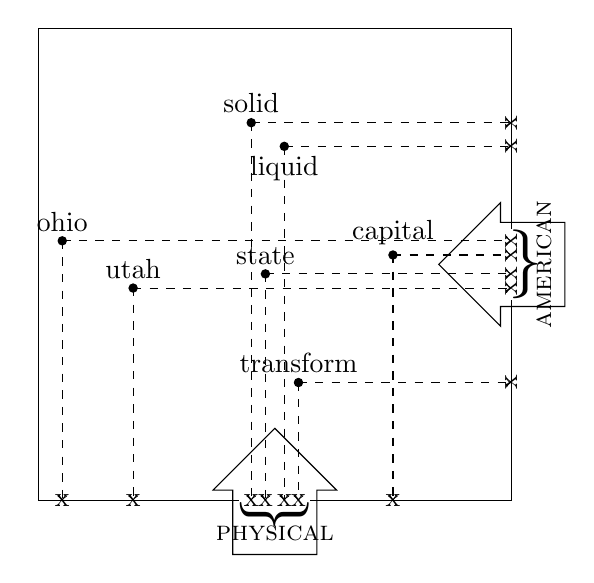
\begin{tikzpicture}[scale=0.06,baseline]
    	\draw (0,0)--(-100,0)--(-100,-100)--(-57.5,-100);
        \draw (-42.5,-100)--(0,-100)--(0,-57.5);
        \draw (0,-42.5)--(0,0);

    	\draw (-52,-52) [above] node {state};
        \fill (-52,-52) circle[radius=1];
        \draw[dashed,->] (-52,-52)--(-52,-100);
        \draw (-52,-100) node {x};
        \draw[dashed,->] (-52,-52)--(0,-52);
        \draw (0,-52) node [rotate=90] {x};

    	\draw (-55,-20) [above] node {solid};
        \fill (-55,-20) circle[radius=1];
        \draw[dashed,->] (-55,-20)--(-55,-100);
        \draw (-55,-100) node {x};
        \draw[dashed,->] (-55,-20)--(0,-20);
        \draw (0,-20) node [rotate=90] {x};

    	\draw (-25,-48) [above] node {capital};
        \fill (-25,-48) circle[radius=1];
        \draw[dashed,->] (-25,-48)--(-25,-100);
        \draw (-25,-100) node {x};
        \draw[dashed,->] (-25,-48)--(0,-48);
        \draw (0,-48) node [rotate=90] {x};

    	\draw (-48,-25) [below] node {liquid};
        \fill (-48,-25) circle[radius=1];
        \draw[dashed,->] (-48,-25)--(-48,-100);
        \draw (-48,-100) node {x};
        \draw[dashed,->] (-48,-25)--(0,-25);
        \draw (0,-25) node [rotate=90] {x};
        
        \draw (-45,-75) [above] node {transform};
        \fill (-45,-75) circle[radius=1];
        \draw [dashed,->] (-45,-75)--(-45,-100);
        \draw (-45,-100) node {x};
        \draw [dashed,->] (-45,-75)--(0,-75);
        \draw (0,-75) node [rotate=90] {x};
        
        \draw (-80,-55) [above] node {utah};
        \fill (-80,-55) circle[radius=1];
        \draw [dashed,->] (-80,-55)--(-80,-100);
        \draw (-80,-100) node {x};
        \draw [dashed,->] (-80,-55)--(0,-55);
        \draw (0,-55) node [rotate=90] {x};
        
        \draw (-95,-45) [above] node {ohio};
        \fill (-95,-45) circle[radius=1];
        \draw [dashed,->] (-95,-45)--(-95,-100);
        \draw (-95,-100) node {x};
        \draw [dashed,->] (-95,-45)--(0,-45);
        \draw (0,-45) node [rotate=90] {x};
        
        \node at (3,-50) {\Huge\}};
        \node at (-50,-103) [rotate=-90] {\Huge\}};
%        \node at (-50,-103) [rotate=-90] {\fontsize{80pt}{4em}\selectfont \}};
        
        \node at (-50,-102.5) [single arrow,draw,rotate=90,minimum height=40,minimum width=40,inner sep=15] {};
        \node at (-50,-107) {\textsc{physical}};
        \node at (2.5,-50) [single arrow,draw,rotate=180,,minimum height=40,minimum width=40,inner sep=15] {};
        \node at (7,-50) [rotate=90] {\textsc{american}};
    \end{tikzpicture}
    \end{subfigure}
    \caption{An ambiguous two-dimensional space of words relating to the term \emph{cat} (a), and a refined space where, based on two different one-dimensional projections, two different conceptual mappings of \emph{cat} emerge as word clusters (b).}
\end{figure}

\section{A Literal, Dynamic Language Model}

The model described here is characterised by two crucial features:

\begin{enumerate}
\item The dimensional features of the space are literally interpretable, in that they correspond to information theoretical statistics about the co-occurrence of words in a large scale corpus.
\item Following on this first point, the model operates by a procedure of continuously unfolding projections of subspaces, with the character of these projections determined by a continuous dimensional analysis based on input terms.
\end{enumerate}

In the first instance, the maintenance of dimensions populated by statistics pulled directly from a corpus traversal differentiates this approach from recent work by the likes of \cite{MikolovEA2013b} and \cite{PenningtonEA2014}, who have made use of neural networks and matrix factorisation to build models which perform well on hand-crafted test sets designed to test the models' performance on specific aspects of conceptualisation.  It is precisely the statistically concrete nature of the present model which allows it to remain conceptually dynamic.  Because the model's dimensions correspond literally to co-occurrence terms, an analysis of the dimensions that contribute strongly to terms observed as occurring in a particular contextual context can be drawn out and used to project a subspace from a base model.

\section{The Geometry of Metaphor}
The contextual dynamism of concepts is implicit in the isomorphic mappings between conceptual schemes at the root of \citepos{Lakoff} conceptual metaphors.  It is the internal anatomy of each conceptual scheme, produced by the environmental and consequent cultural entanglements inherent in language, that allows the alignment of conceptual schemes: there is always an implicit geometric foundation to these mappings (and this foundation is often rather more explicit, as in the case of, for example, orientation and conduit metaphors).  This project seeks to realise a practical implementation of this theoretical stance, in particular by utilising the geometric qualities of the contextualised subspaces that have already been described.  In particular, the al

There is once again a point of comparison with the models that have been described in the contemporary NLP literature here.  The analogy completions performed by the model of, for instance, \cite{MikolovEA2013b} employ a clever layer of basic linear algebra to word-vectors derived through the complex non-linear processing of corpus data.  These operations are, however, dependent on a certain consistency of scale within a space.  The algebraic relationship $\overrightarrow{king}-\overrightarrow{queen} = \overrightarrow{man}-\overrightarrow{woman}$, for instance, which has been discussed extensively in recent papers, depends on a comparability not only in terms of orientation but also in terms of distance between the spaces of \textsc{royals} and \textsc{people}.  This is a special category of analogy within a distributional model, however, as there are demonstrably comparable conceptualisations mappable from word clusterings of various scales.

By instead relying on the general geometric property of congruity rather than the specific scale of a space, the model described here offers a more robust approach to drawing connections between spaces.  If a concept is represented as a cluster of words that emerge in a distributional semantic subspace, then the theory here is that there should be mappings between the words in two different such subspaces which, taken as a whole, substantiate a conceptual metaphor.  The intuition here can be related to a more traditional transference view of metaphor: there will be some notable overlap between the co-occurrence profiles of the respective distributional spaces of, for instance, \textsc{surgery} and \textsc{butchery}.  By identifying this overlap, it should be possible to draw out correspondences between conceptual components such as \emph{scalpel} and \emph{cleaver}, and this in turn allows for the postulation of an alignment between the spaces which represents a metaphor.  Thus it is the geometry of the spaces which ultimately affords the opportunity for constructing a new semantic connection between conceptual domains, and the evident transference of intensions might be interpreted as an \emph{a posteriori} logical artefact of this process.

\begin{figure}
	\centering
	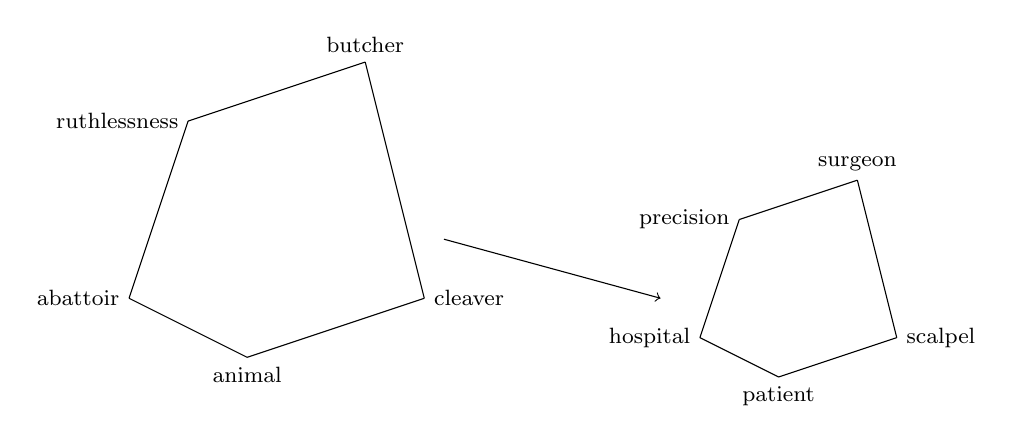
\begin{tikzpicture}[scale=0.25]
		\draw (6,15)--(15,18) node [above] {\footnotesize butcher};
		\draw (15,18)--(18,6) node [right] {\footnotesize cleaver};
		\draw (18,6)--(9,3) node [below] {\footnotesize animal};
		\draw (9,3)--(3,6)node [left] {\footnotesize abattoir};
		\draw (3,6)--(6,15) node [left] {\footnotesize ruthlessness};
		
		\draw [->] (19,9)--(30,6);
		
		\draw (34,10)--(40,12) node [above] {\footnotesize surgeon};
		\draw (40,12)--(42,4) node [right] {\footnotesize scalpel};
		\draw (42,4)--(36,2) node [below] {\footnotesize patient};
		\draw (36,2)--(32,4) node [left] {\footnotesize hospital};
		\draw (32,4)--(34,10) node [left] {\footnotesize precision};
	\end{tikzpicture}
	\caption{Congruences discovered in subregions of a vector space model suggest metaphoric mappings.  The regions do not necessarily have to be of the same scale in order to identify a possible alignment.}
\end{figure}

\chapter{Methodology}

\section{A Lexical Base Model}
The general model is trained by a single traversal of a large scale corpus.  Token by token, co-occurrence frequencies are tabulated for each word type, and the dimensions of the model are populated with information theoretical statistics measuring the mutual information associated with the observation of a context word occurring within a window of a certain number of words from a vocabulary word.  The result is a matrix with rows corresponding to word-vectors and columns corresponding to co-occurrence terms, such that an element $M_{w,c}$ measures the mutual information inherent in the co-occurrence of term $c$ with word $w$, where $N$ is the total count of word tokens in the corpus, $n_{w,c}$ is the frequency with which $c$ occurs in the context window of $w$, $n_w$ is the total frequency of word $w$, $n_c$ is the total count of times that $c$ is observed in the context of another word, and $a$ is a smoothing constant:

\begin{equation}\label{eq:MI}
M_{w,c} = \log_2 \left(\frac{n_{w,c} \times N}{n_w \times \left(n_c + a\right)} + 1\right)
\end{equation}

Once this base space is established, a dimensional analysis of input terms provides the basis for the projection of contextually informed subspaces.  So, for instance, given an input of terms $w_1$, $w_2$, and $w_3$, the model analyses the corresponding word-vectors $\overrightarrow{w_1}$, $\overrightarrow{w_2}$, and $\overrightarrow{w_3}$ to determine the salient co-occurrence dimensions shared between all three terms, which is to say, those universally non-zero dimensions with the highest mean value.  These dimensions are then used as the basis for the generation of a subspace, with the expectation that conceptually relevant terms will emerge in this new, significantly lower-dimensional space.  In particular, conceptual constituents are identified by searching for word-vectors that cluster around a positive central point considerably removed from the origin, by searching for the word-vectors with the greatest norms, and by searching for the word-vectors that are, on average, furthest away in terms of Euclidean distance from any other word vectors.

\section{Taxonomy Recapitulation}
The conceptual projections of the lexical base model perform particularly well at extending the membership of short lists of words corresponding to constituents of some conceptual category (so, for instance, a list containing \emph{lion}, \emph{tiger}, and \emph{bear} is expanded to include other exemplars of the concept \textsc{wild animal}).  With this in mind, a mechanism for establishing hypernymic relationships between such lists and terms denoting a general categorisation of such lists should lead to the effective reconstruction of hand-crafted lexical ontologies such as WordNet.

The proposed way forward at the time of writing is to establish a technique for analysing the co-occurrence data for singular terms and then to generate short lists of other words as candidates for list expansion operations.  This will most likely involve inspecting potential groupings of the terms that emerge from a subspace for high degrees of mutual co-occurrence, and then expanding top scoring sets to discover potential groupings of terms to be considered as constituents of a certain conceptual subtree.  There will also have to be a system for maintaining and then eventually comparing hypotheses about the conceptual relationships between the denotations of word pairs, as well as a mechanism for ultimately resolving these hypotheses into a well formed ontology.

\section{Analogy Completion}
Where work from researchers such as \cite{Mikolov}, \cite{Pennington}, and \cite{Levy} has focused on building distributional semantic spaces where simple arithmetical operations between word-vectors yield good results for certain types of analogies, the project presented here will focus on more robustly geometric methods to identify congruences between different contextualised projections.  As a first pass at this problem, searching for word-vectors that complete basic geometric transformations within a space seems like a viable approach to this task.  So, for instance, there is some transformation from the space of \textsc{butchery} to the space of \textsc{surgery} that preserves the overlapping co-occurrence relationships between words like \emph{cleaver} and \emph{scalpel} while aligning the 

\section{Metaphor Generation}
The ultimate goal of metaphor generation will involve a kind of reverse engineering of the model's approach to analogy completion: once the mechanism for performing analogical transformations between conceptually rooted word-subspaces has been refined, these transformations can be applied to a given projection based on the dimensional information inherent in the influence of some contextualising term.  Once these transformations are applied, the relatively sparse transformed source space can be searched for the points that best align with the geometry of the target space.

\chapter{Implementation and Results}
The base model has been trained on the English language text of Wikipedia, compiling statistics for a vocabulary of the 200,000 most frequent word types in the corpus and the terms that occur within a window of five words on either side of each token of the elements of the vocabulary.  In the cases presented here, the 200 most salient dimensions for each input query are used to project the contextualised subspaces.

\section{The Base Model and Projections}
Tests performed so far on the base model have returned good results for some sample contextual projections from the base model.  Two different types of input queries have been considered, one involving terms which together denote some contextually specific concept and another which offers a short list of conceptual exemplars.  Results for four sample queries are offered in~\ref{tab:context}, with the top ten output words in terms of norm being reported.

\begin{center}
	\begin{table}[h]\small
	\caption{Contextualised Word Spaces}
	\label{tab:context}
	\centering
	\begin{tabular}{|l|l|l|l|}
		\hline
		\multicolumn{2}{|c|}{\textsc{by hypernym}} & \multicolumn{2}{c|}{\textsc{by list}} \\
		\hline
		\multicolumn{1}{|c|}{\emph{wild animals}} & \multicolumn{1}{c|}{\emph{professional occupations}} & \multicolumn{1}{c|}{\emph{lion,tiger,bear}} & \multicolumn{1}{c|}{\emph{surgeon,butcher,builder}} \\
		\hline
		pocupines & technicians & leopard & bricklayer \\
		deer & accountants & dhole & grocer \\
		boar & technologists & hyena & apprenticed \\
		rabbits & therapists & boar & wheelwright \\
		foxes & electricians & langur & blacksmith \\
		raccoons & physiotherapists & macaque & plumber \\
		boars & dentists & tapir & shoemaker \\
		goats & hygienists & chital & industrialist \\
		squirrels & pharmacists & lion & joiner \\
		hares & nurses & rhinoceros & cabinetmaker \\
		\hline
	\end{tabular}
	\end{table}
\end{center}

\section{Taxonomies}
Some preliminary results, comparing the performance of the model described here versus the word2vec model of \cite{Mikolov}, are offered in~\ref{tab:hyper}.  The linear algebraic technique of using vector addition and then rating similar terms based on cosine similarity has been applied in the case of word2vec, as described in the literature.  Here \emph{hits} refer to terms that can be found in the WordNet subtree of terms associated with the appropriate synset for each input query, \emph{misses} refer to terms that are in WordNet but are not in the appropriate subtree, \emph{absent} tallies terms that are not in WordNet at all, and \emph{duplicate} indicates the count of terms that are morphemically identical to other words already returned by each model.

\begin{center}
	\begin{table}[h]\small
	\caption{Comparative Hypernymy}
	\label{tab:hyper}
	\centering
	\begin{tabular}{|r|l|l|l|l|}
		\cline{2-5}
		\multicolumn{1}{c|}{} & \multicolumn{2}{c|}{\emph{wild animals}} & \multicolumn{2}{c|}{\emph{visual artist}} \\
		\cline{2-5}
		\multicolumn{1}{c|}{} & \multicolumn{1}{c|}{\textsc{model}} & \multicolumn{1}{c|}{\textsc{w2v}} & \multicolumn{1}{c|}{\textsc{model}} & \multicolumn{1}{c|}{\textsc{w2v}} \\
		\hline
		\textsc{hits} & 40 & 34 & 16 & 8 \\
		\textsc{misses} & 5 & 9 & 24 & 30 \\
		\textsc{absent} & 2 & 2 & 7 & 9 \\
		\textsc{duplicate} & 3 & 5 & 3 & 3 \\
		\hline
	\end{tabular}
	\end{table}
\end{center}

\section{Analogies}
Preliminary experiments have been carried out to explore the comparative geometry of different word-spaces.  The approach thus far has been to measure the angles of the vertexes of different constellations of word-vectors within a subspace, and then to examine how these angles line up with the angles in another space with an eye towards describing a prospective conceptual mapping.  Experiments with the model's projections are under way, and results will be forthcoming.  For the time being, \ref{tab:metaphors} offers a comparison between terms within the general, non-reduced space.  Three mappings are offered; in each case, all possible alignments of words between each space are compared.  The average difference in angle between each of the two spaces for each possible alignment is calculated, and the ranking of the alignment that is deemed, for the purposes of this test run, conceptually satisfactory as compared to all other alignments is returned.  The high performance of the appropriate alignments even in the unrefined base space motivates further and more rigorous testing of mappings between projected spaces, which should remit a much higher degree of conceptual coherence.

\begin{table}[h]\footnotesize
\centering
\caption{Angular Mappings of Conceptual Regions}
\label{tab:metaphors}
	\begin{tabular}{|l||l|l|l|}
		\hline
		target & ROYALS & SURGERY & EMOTIONS \\
		source & PEOPLE & BUTCHERY & ORIENTATIONS \\
		\hline
		rank & 1 out of 24 & 15 out of 720 & 3 out of 720 \\
		mean & 0.062 & 0.046 & 0.048 \\
		high & - & 0.037 & 0.045 \\
		low & 0.198 & 0.094 & 0.101 \\
		\hline
		\multirow{6}{*}{mappings} & man $\rightarrow$ king & butcher $\rightarrow$ surgeon & up $\rightarrow$ happiness \\
			&woman $\rightarrow$ queen & cleaver $\rightarrow$ scalpel & down $\rightarrow$ sadness \\
			&boy $\rightarrow$ prince & abattoir $\rightarrow$ hospital & out $\rightarrow$ loneliness \\
			&girl $\rightarrow$ princess & lamb $\rightarrow$ patient & in $\rightarrow$ togetherness \\
			&& pig slaught. $\rightarrow$ operation & atop $\rightarrow$ control \\
			&& ruthlessness $\rightarrow$ precision & beneath $\rightarrow$ incapacity \\
		\hline
	\end{tabular}
\end{table}

\chapter{Evaluation}
This section for now very broadly outlines some of the evaluative objectives of this project.

but the crucial

considered here is the necessity of resorting to some real world mechanisms for assessing the model's performance, both through formal studies with human subjects and through a less structured but more public testing of the system 

\section{Taxonomy and Analogy}
One problem inherent in the use of datasets, be they test sets specifically designed to examine features of computational language models or general and highly public frameworks such as WordNet or DBpedia, is the necessarily biased and incomplete process of assigning conceptual relationships to senses of words.  As such, in addition to the straightforward analysis of results over test sets and reporting of precision, recall, and related statistics for ontology recapitulation, it will probably be necessary to resort to asking human subjects about the efficacy of the model's conceptual mappings.

\section{Metaphor}
Even more than with the only moderately controversial tasks of determining whether conceptual and analogical relationships are appropriately captured by the models output, the problem of assessing the creative value of metaphoric artefacts generated by the model is fraught with the 

In the end, the criteria of usefulness and novelty generally taken as the basic standard for computationally creative output can serve as a good guide for the model's target, but not as much more than this.  Simply asking humans whether they consider the model to be performing along these lines must be a hopelessly subjective enterprise

\chapter{Conclusion}


\bibliographystyle{apacite}
\bibliography{/home/masteradamo/academy/Cite.bib}

% Start the appendix (inc. author's publications)
\begin{appendix}
%\chapter{Author's publications}

% publications goes here

\subsection*{Journal papers}
\begin{enumerate}
  \item \textbf{Y. Gao}, X. Chen, Z. Ying and C. G. Parini, ``Design and Performance
Investigation of a Dual-element PIFA Array at 2.5 GHz for MIMO Terminals," \emph{IEEE Trans. on
Antennas and Propagation}. (Revising)

\end{enumerate}


\subsection*{Conference papers}


\begin{enumerate}
  \item \textbf{Y. Gao}, X. Chen, Z. Ying and C. G. Parini , ``Further Investigation of a
Dual-Element Diversity PIFA for MIMO Applications at 2.5 GHz Band," \emph{IEEE International
Symposium on Antennas and Propagation (AP-S)} , Honolulu, Hawaii, USA  June, 2007. (Accepted)
    
\end{enumerate}

\subsection*{Project report}
\begin{enumerate}
  \item X. Chen and \textbf{Y. Gao}, ``Final Report on Modelling of Difficult Environments,"
  Galileo Advance Concept project final report (GAC/EUT/DT/219), 9th June - 31 October 2007.
  
\end{enumerate}



\renewcommand{\thefigure}{B.\arabic{figure}}
\chapter{Solutions for the Examples in Chapter 2}
\label{examples_solutions}
\section{Example 1: Antenna Spacing Effect}

\textbf{Step 1:} Get the $H_{norm}H_{norm}^\dagger$, set $2{\pi}R/\lambda={\omega}_1$ and
$2{\pi}(\overline{R})/\lambda={\omega}_2$ ($\lambda$ is the wavelength), so
\begin{equation}
H_{norm} = \frac{1}{\sqrt 2 }\left( {{\begin{array}{*{20}c}
 {e^{ - j\omega _1 }} \hfill & {e^{ - j\omega _2 }} \hfill \\
 {e^{ - j\omega _2 }} \hfill & {e^{ - j\omega _1 }} \hfill \\
\end{array} }} \right)
\end{equation}
Note: $H_{norm}^\dagger=(\overline{H_{norm}})^T$ and $e^{j\theta}=cos\theta +jsin\theta$
\begin{equation}
\begin{array}{l}
 H_{norm}H_{norm}^\dagger = \frac{1}{2}\left( {{\begin{array}{*{20}c}
 {e^{ - j\omega _1 }} \hfill & {e^{ - j\omega _2 }} \hfill \\
 {e^{ - j\omega _2 }} \hfill & {e^{ - j\omega _1 }} \hfill \\
\end{array} }} \right)\left( {{\begin{array}{*{20}c}
 {e^{j\omega _1 }} \hfill & {e^{j\omega _2 }} \hfill \\
 {e^{j\omega _2 }} \hfill & {e^{j\omega _1 }} \hfill \\
\end{array} }} \right) \\
 = \frac{1}{2}\left( {{\begin{array}{*{20}c}
 {1 + 1} \hfill & {e^{ - j(\omega _1 - \omega _2 )} + e^{ - j(\omega _1 -
\omega _2 )}} \hfill \\
 {e^{ - j(\omega _1 - \omega _2 )} + e^{ - j(\omega _1 - \omega _2 )}}
\hfill & {1 + 1} \hfill \\
\end{array} }} \right) \\
 = \left( {{\begin{array}{*{20}c}
 1 \hfill & {\cos (\omega _1 - \omega _2 )} \hfill \\
 {\cos (\omega _1 - \omega _2 )} \hfill & 1 \hfill \\
\end{array} }} \right) \\
 \end{array}
\end{equation}
\textbf{Step 2:} Get the eigenvalue of $H_{norm}H_{norm}^\dagger$, here set $\lambda$ as
eigenvalue, then,
\begin{equation}
\left( {{\begin{array}{*{20}c}
 {1 - \lambda } \hfill & {\cos (\omega _1 - \omega _2 )} \hfill \\
 {\cos (\omega _1 - \omega _2 )} \hfill & {1 - \lambda } \hfill \\
\end{array} }} \right) = 0
\end{equation}
and $\omega_1-\omega_2=2{\pi}R/\lambda-2{\pi}(\overline{R})/\lambda=-54^o$, so
$\lambda=1{\pm}cos(\omega_1-\omega_2){\approx}1{\pm}0.59$. Hence, $\lambda_1=1.59$ and
$\lambda_2=0.41$.





\end{appendix}

\end{document}
% That's all of it!
